\documentclass[border=3pt]{standalone}
\usepackage{tikz}
\usepackage{amsmath}
\usepackage{amssymb}
\usepackage{ctex}
\usetikzlibrary{matrix, calc, positioning}
\usepackage{pgfplots}
\pgfplotsset{compat=1.18}

\begin{document}

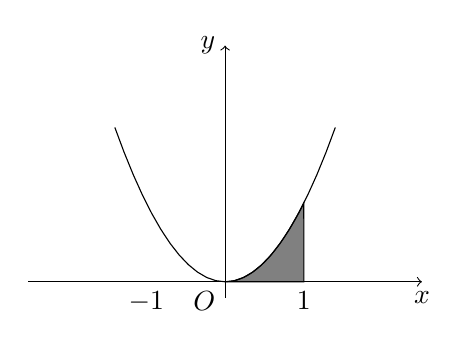
\begin{tikzpicture}
	\draw[->](-2.5,0)--(2.5,0)node[below]{$x$};
	\draw[->](0,-0.2)--(0,3)node[left]{$y$};
	\node[below left]at(0,0){$O$};
	\draw[fill=gray,domain=0:1] (0,0) -- plot({\x},{(\x)^2}) -- (1,0) -- cycle;
	\draw[domain=-1.4:1.4] plot({\x}, {(\x)^2});
	\node[below]at(1,0){$1$};
	\node[below]at(-1,0){$-1$};
\end{tikzpicture}

\end{document}
